\section{Требования к системе}

\subsection{Характеристика объекта автоматизации}

Цель дипломного проекта~-- разработка комплексной системы управления офисными информационными процессами, обеспечивающей интеграцию и автоматизацию различных аспектов организации рабочего пространства в условиях распределённых офисных локаций. Система обеспечивает единую точку входа для всех задач сотрудников, их менеджеров, а также интеграцию со сторонними системами. Основная цель системы~-- повышение эффективности управления офисными ресурсами. В основе проекта лежит создание единой информационной платформы и её интеграция с техническими устройствами, что позволяет обеспечить высокую производительность, масштабируемость и надёжность серверной части системы. Проект предусматривает детальную проработку бизнес-процессов, включающих бронирование рабочих мест, оборудования, переговорных и коворкинговых комнат, а также автоматическую рассадку сотрудников и контроль доступа в помещения.

Системный анализ процессов с применением методов моделирования позволяет оптимизировать маршруты взаимодействия между модулями системы, повысить скорость принятия решений и минимизировать человеческий фактор в рутинных операциях. Алгоритмы автоматической рассадки сотрудников, построенные на основе методов оптимизации, обеспечивают равномерное распределение персонала, минимизируя затраты времени на организацию рабочего процесса. Помимо этого, система автоматизированного контроля доступа, реализованная через выдачу прав на доступ, предусматривает интеграцию с техническими средствами идентификации – от персональных карточек до биометрических систем распознавания отпечатков и лиц. Это позволит оптимизировать управленческую и аналитическую деятельность предприятия.


\subsection{Разработка функциональных требований}
\label{sec:tech-requirements:functional-requirements}

Функциональные требования (набор сценариев) описывают различное поведение системы в зависимости от входных данных и зависят от типа разрабатываемой системы и
потребностей пользователей.


\textit{\textbf{Модуль управления офисными ресурсами}} должен обеспечивать сотрудникам возможность бронировать рабочие места с учетом их предпочтений и временных интервалов, а также предоставлять менеджерам инструменты для утверждения запросов и автоматической рассадки сотрудников. Все процессы должны быть максимально автоматизированы для минимизации ручного вмешательства. Разрабатываемая система должна предоставлять пользователям осуществлять следующие действия:

\begin{enumerate}
    \item \textit{Создание запроса на бронирование рабочего места}. Система должна предоставлять возможность сотруднику создавать запрос на бронирование рабочего места. Запрос должен включать:
        \begin{itemize}
            \item выбор офиса, этажа, комнаты и конкретного рабочего места;
            \item указание временного интервала бронирования (временное или постоянное);
            \item возможность указания дополнительных предпочтений (например, близость к окну, тихая зона).
        \end{itemize}

    \item \textit{Утверждение (отклонение) запроса на бронирование} рабочего места менеджером или сотрудником с соответствующими правами. После утверждения запроса система должна автоматически обновлять статус рабочего места как занятого.

    \item \textit{Просмотр доступных рабочих мест} в выбранном офисе, этаже или комнате с фильтрацией по различным параметрам (например, доступность, тип рабочего места).

    \item \textit{Автоматическая рассадка сотрудников}. Система должна автоматически распределять сотрудников по рабочим местам на основе заданных параметров (например, предпочтения сотрудников, доступность мест). Возможность ручной корректировки автоматической рассадки менеджером.
\end{enumerate}

Кроме того, в рамках модуля предполагается наличие функциональности для управления оборудованием, которая должна позволять сотрудникам бронировать оборудование, как переносное, так и стационарное, с указанием временного интервала и дополнительных параметров. Менеджеры должны иметь возможность утверждать запросы и контролировать доступность оборудования, обеспечивая его эффективное использование. Это включает в себя реализацию следующих возможностей:

\begin{enumerate}
    \item \textit{Создание запроса на бронирование оборудования}. Запрос должен включать:
        \begin{itemize}
            \item выбор типа оборудования (переносное или непереносное);
            \item указание временного интервала бронирования;
            \item возможность указания дополнительных параметров (например, необходимость доставки оборудования).
        \end{itemize}

    \item \textit{Утверждение (отклонение) запроса на бронирование оборудования} менеджером или сотрудником с соответствующими правами. После утверждения запроса система должна автоматически обновлять статус оборудования как занятого.

    \item \textit{Просмотр доступного оборудования} в выбранной локации с возможностью фильтрации по различным параметрам (например, тип оборудования, доступность).
\end{enumerate}

Также модуль должен предоставлять возможность для автоматизированной генерации отчетов по использованию рабочих мест, оборудования и времени нахождения сотрудников в помещениях, а также предоставлять инструменты для визуализации данных в виде графиков и диаграмм. Это позволит анализировать эффективность использования офисных ресурсов и принимать обоснованные управленческие решения.


\textit{\textbf{Модуль управления сотрудниками}} предполагает наличие функциональности для администрирования сотрудников предприятия. К конкретным требованиям относятся следующие функциональные возможности:

\begin{itemize}
    \item создание, обновление и удаление сотрудников предприятия;
    \item создание, обновление и удаление персональных идентификаторов сотрудников для дальнейшей их интеграции с модулем контроля посещаемости;
    \item автоматизированное ведение журнала истории действий пользователей в системе;
    \item управление иерархией сотрудников предприятия, путем назначения сотрудников к департаментам (отделам), указание профессионального уровня и занимаемой должности.
\end{itemize}


\textit{\textbf{Модуль контроля доступа}} должен интегрироваться с техническими средствами контроля доступа, такими как карты и биометрические системы, для автоматической идентификации сотрудников и управления их доступом в помещения. Учет времени нахождения сотрудников в помещениях и генерация соответствующих отчетов также должны быть реализованы. Это включает в себя наличие следующих возможностей:

\begin{enumerate}
    \item \textit{Управление доступом в помещения}. Система должна предоставлять возможность менеджерам или сотрудникам с соответствующими правами выдавать права доступа в помещения (постоянный или временный доступ) с автоматическим обновлением статуса доступа сотрудника в зависимости от выданных прав.

    \item \textit{Интеграция с техническими средствами контроля доступа}, такими как считыватели персональных карт, биометрические сканеры отпечатков пальцев и системы распознавания лиц. Система должна автоматически идентифицировать сотрудников и управлять их доступом в помещения на основе их роли и прав.

    \item \textit{Отслеживание и учет времени нахождения сотрудников в помещениях} с возможностью генерации различных отчетов по заданным параметрам.
\end{enumerate}


\textit{\textbf{Модуль уведомлений}} предоставляет возможности для автоматизированной отправки уведомлений и рассылок сотрудникам. События, которые вызывают отправку уведомлений, могут вызываться в ручном режиме администраторами системы, или генерироваться автоматически путем выполнения определенных действий в системе, например, утверждении или отклонении запроса на бронирование, выпуск нового персонального идентификатора и тд.

Схема взаимодействия модулей системы приведена на рис.~\ref{fig:tech-requirements:functional-requirements:schema-of-modules}.

\begin{figure}[h]
\centering
    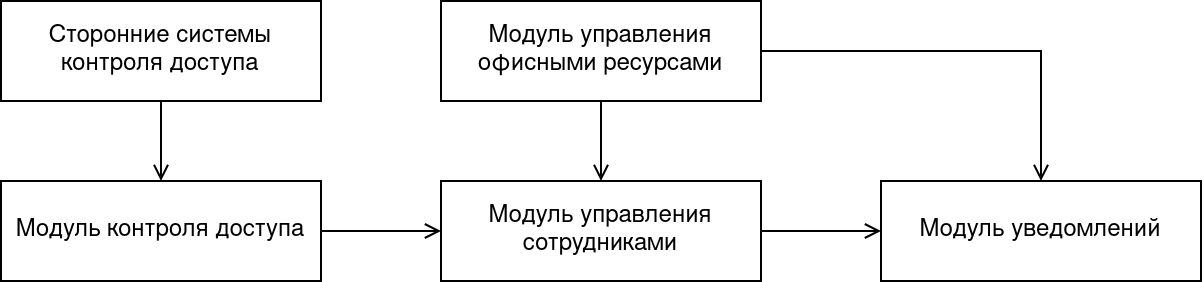
\includegraphics[width=0.9\linewidth]{assets/schema-of-modules.png}
    \caption{Схема взаимодействия модулей системы}
    \label{fig:tech-requirements:functional-requirements:schema-of-modules}
\end{figure}


\subsection{Разработка нефункциональных требований}

Нефункциональные требования описывают атрибуты качества системы, такие как производительность, безопасность, удобство использования и другие характеристики, которые не связаны напрямую с функциональностью, но критически важны для успешной работы системы. Ниже представлены нефункциональные требования для разрабатываемой системы управления офисными информационными процессами.

\begin{enumerate}
    \item \textit{Производительность и масштабируемость}.
        \begin{itemize}
            \item время отклика системы должно составлять не более 2 секунд для 95\% запросов при средней нагрузке и при использовании среднестатистического ADSL Интернет-соединения;
            \item наличие возможностей горизонтального масштабирования для увеличения производительности при росте числа пользователей, что позволит достичь обработки до 10 000 одновременных пользователей без снижения производительности;
            \item нагрузочная устойчивость системы должна обеспечивать полную работоспособность при пиковых нагрузках, например, в начале рабочего дня, когда большинство сотрудников пытаются забронировать рабочие места или оборудование.
        \end{itemize}

    \item \textit{Безопасность}.
        \begin{itemize}
            \item поддержка многофакторной аутентификации для сотрудников. Доступ к функциональности системы должен быть строго регламентирован на основе ролей и прав пользователей. Все личные данные сотрудников, если таковые имеются, должны быть недоступны никому кроме пользователей и администраторов системы;
            \item защита и шифровка передаваемых данных между клиентом и сервером должна быть обеспечена использованием протокола HTTPS. Конфиденциальные данные, такие как биометрическая информация, пароли, и прочая чувствительная ко взлому информация, должны храниться в зашифрованном виде;
            \item журнал всех действий пользователей для последующего аудита должен формироваться в автоматическом режиме для последующей реализации механизмов мониторинга для выявления и предотвращения несанкционированного доступа.
        \end{itemize}

    \item \textit{Удобство использования}.
        \begin{itemize}
            \item интерфейс системы должен быть интуитивно понятным и простым в использовании, с минимальным временем обучения для новых пользователей и поддержкой адаптивного дизайна для корректного отображения на различных устройствах (ПК, планшеты, смартфоны);
            \item наличие возможностей для последующего внедрения поддержки нес\-коль\-ких языков для удобства использования в международных офисах компании;
            \item совместимость с основными операционными системами (\textit{Win\-dows}, \textit{macOS}, \textit{Linux}) и браузерами (\textit{Chrome}, \textit{Firefox}, \textit{Safari}, \textit{Edge}).
        \end{itemize}

    \item \textit{Надежность и отказоустойчивость}.
        \begin{itemize}
            \item доступность системы должна составлять минимум 95\% в течение года;
            \item регулярное резервное копирование данных должно выполняться в автоматическом режиме для обеспечения возможности восстановления в течение 1 часа после сбоя;
        \end{itemize}

    \item \textit{Техническая поддержка и обслуживание}.
        \begin{itemize}
            \item система должна поддерживать возможность обновления без прерывания работы пользователей;
            \item полная техническая и пользовательская документация должна быть доступна для всех модулей системы, а также должна регулярно обновляться в соответствии с изменениями.
        \end{itemize}
\end{enumerate}


\subsection{Диаграмма вариантов использования}
\label{sec:tech-requirements:functional-model}

Функциональная модель системы описывает поведение разрабатываемого программного продукта с точки зрения различных ролей пользователей, участвующих во взаимодействии с системой. Одним из основных инструментов для визуализации функциональных возможностей системы является диаграмма вариантов использования, которая отражает связи между актёрами и прецедентами (сценариями взаимодействия с системой).

Исходя из общей архитектуры системы и анализа требований, были выделены три ключевые роли (актёра):

\begin{itemize}
    \item сотрудник~-- основной пользователь системы, осуществляющий бронирование ресурсов и взаимодействие с функционалом в рамках своей повседневной деятельности;
    \item офис-менеджер~-- ответственен за управление бронированием ресурсов, контроль наличия и состояния оборудования;
    \item менеджер по персоналу~-- осуществляет администрирование пользователей, контроль посещаемости и управление правами доступа.
\end{itemize}

Сотрудник~-- это зарегистрированный пользователь, работающий в офисе на постоянной или временной основе. Основной задачей для данной роли является эффективное планирование и использование офисных ресурсов. Сотрудник взаимодействует с системой через следующие прецеденты:

\begin{enumerate}
    \item Авторизация в системе~-- пользователь проходит процедуру входа с использованием логина и пароля;
    \item Просмотр доступных рабочих мест~-- пользователь получает список свободных мест по выбранным фильтрам (офис, этаж, тип зоны).
    \item Бронирование рабочего места~-- сотрудник выбирает конкретное место, дату и интервал времени, указывает предпочтения (например, ближе к окну).
    \item Просмотр статуса бронирований~-- система отображает активные, завершённые и отклонённые бронирования.
    \item Отмена бронирования рабочего места~-- пользователь имеет возможность отменить ранее созданное бронирование.
    \item Создание запроса на бронирование оборудования~-- формируется заявка на использование ноутбука, проектора или другого инвентаря.
    \item Просмотр расписания оборудования~-- сотрудник может увидеть, в какие дни и часы оборудование занято или свободно.
    \item Запрос на временный доступ в помещение~-- при необходимости доступа к закрытому кабинету или складу, сотрудник отправляет заявку.
    \item Получение уведомлений~-- система информирует о подтверждении/отклонении бронирований, изменениях доступа и других событиях.
    \item Просмотр отчёта о посещаемости~-- сотрудник может ознакомиться со своей историей входов и выходов из помещений.
\end{enumerate}

Диаграмма вариантов использования от имени сотрудника представлена на рис.~\ref{fig:tech-requirements:functional-model:use-cases-employee}.

\afterpage{
    \clearpage
    \begin{landscape}
        \thispagestyle{landscape}
        \begin{figure}[p]
            \centering
            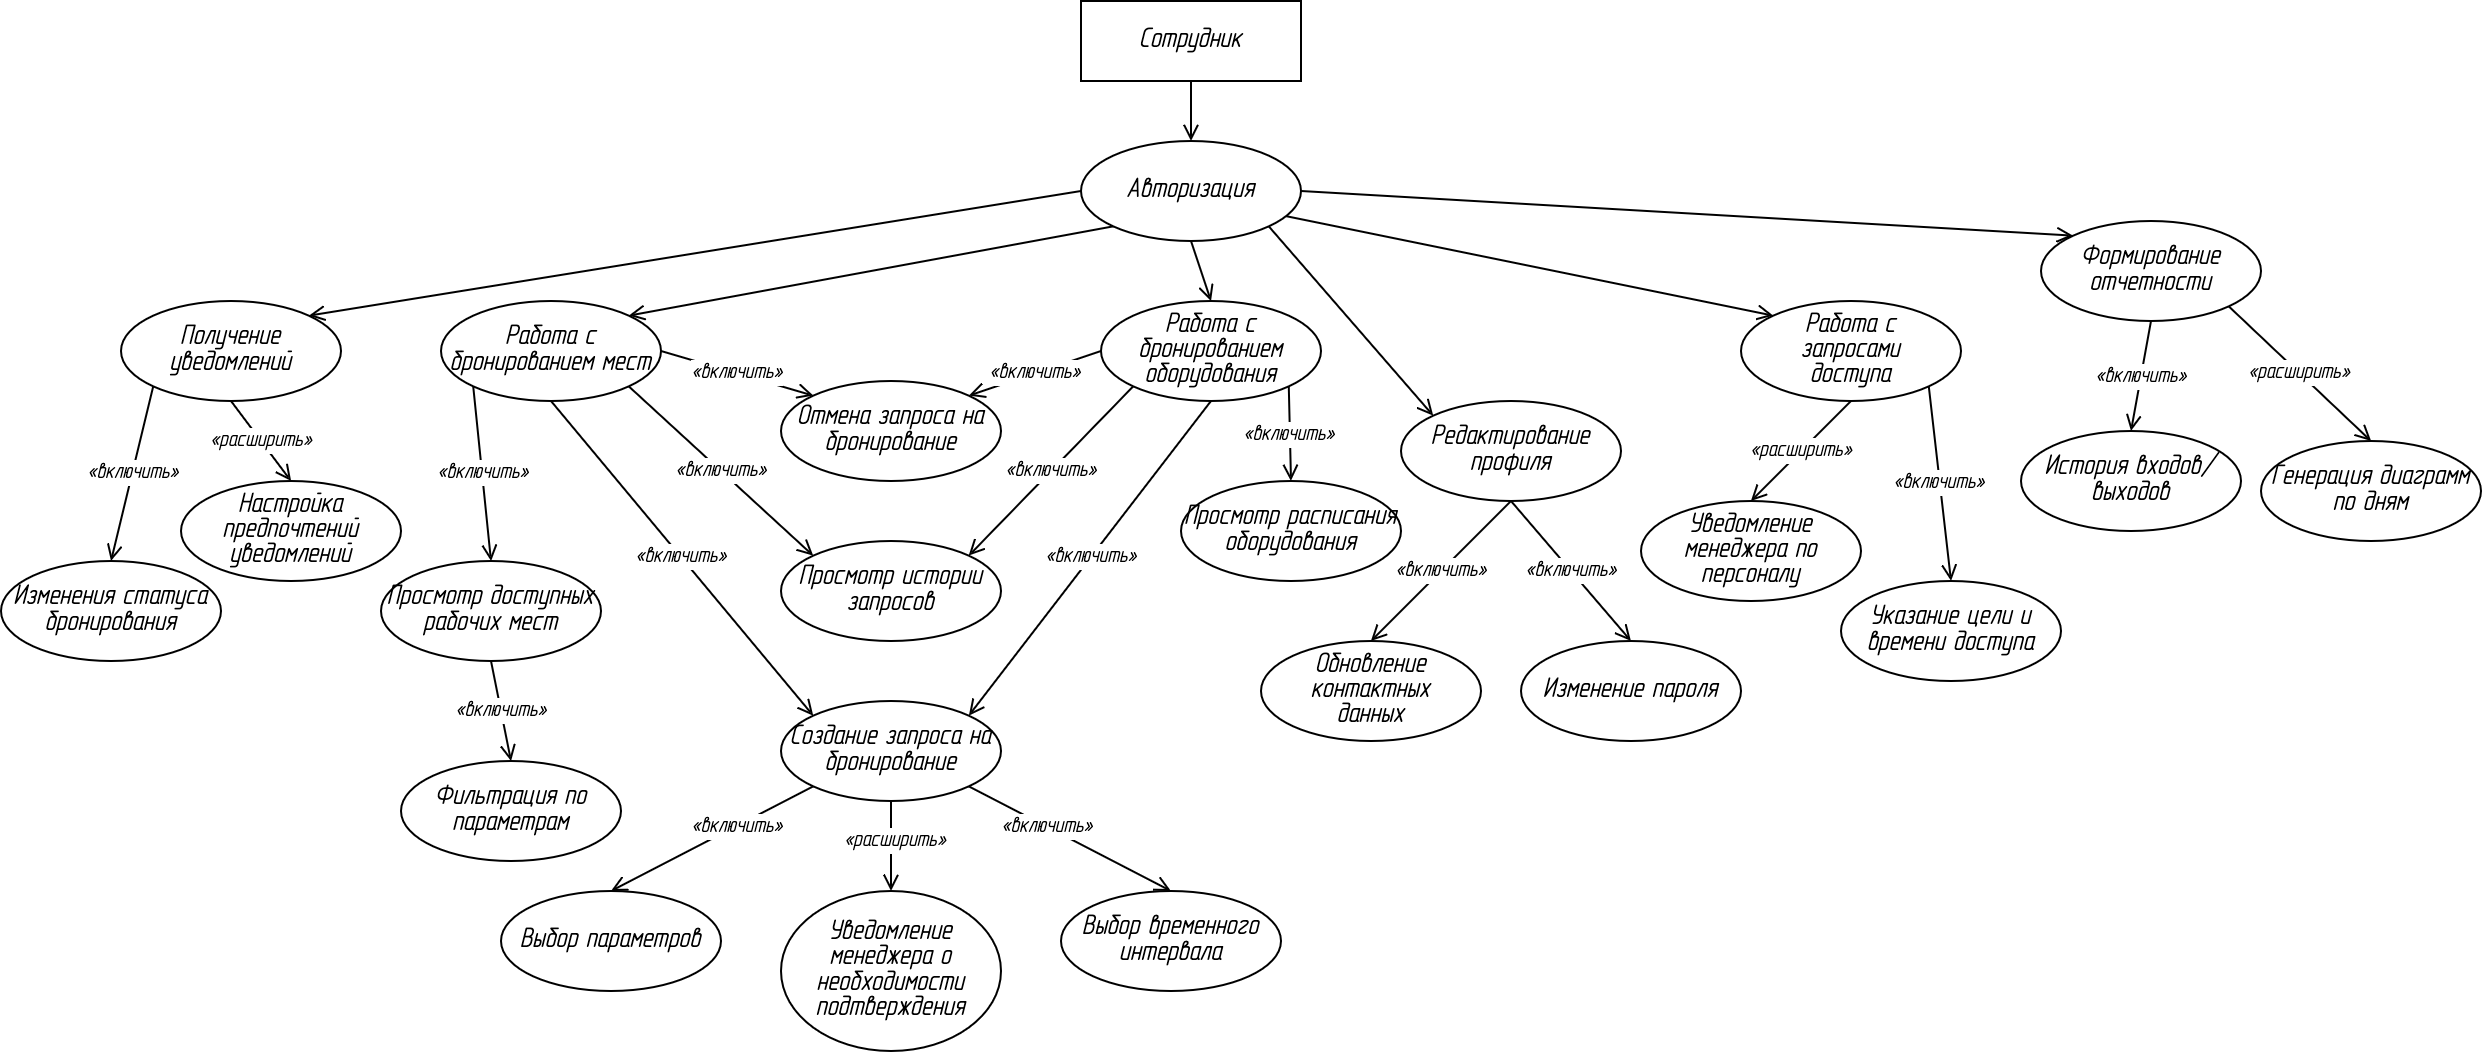
\includegraphics[width=0.99\linewidth]{assets/use-cases-employee.png}
            \caption{Диаграмма вариантов использования от имени сотрудника}
            \label{fig:tech-requirements:functional-model:use-cases-employee}
        \end{figure}
    \end{landscape}
    \clearpage
}

Актёр «Офис-менеджер» в рамках системы выполняет функции административного контроля и технической поддержки сотрудников. Основные задачи этой роли связаны с обработкой заявок на бронирование офисных ресурсов, контролем состояния оборудования и рабочих мест, управлением расписаниями и генерацией отчётности.

Офис-менеджер также после авторизации имеет доступ к набору определенных функций, соответствующих его роли.

\begin{enumerate}
    \item \textit{Обработка заявок на бронирование}~-- ключевая функция офис-ме\-нед\-же\-ра, в рамках которой он получает, просматривает и обрабатывает заявки, созданные сотрудниками на бронирование ресурсов:
    \begin{itemize}
        \item просмотр входящих заявок~-- система предоставляет список всех новых и активных заявок на бронирование;
        \item подтверждение бронирования рабочего места~-- одобрение запроса на использование конкретного рабочего места;
        \item подтверждение бронирования оборудования~-- аналогичная функция для инвентаря, например, ноутбуков или проекторов;
        \item уведомление сотрудника о принятом решении~-- система автоматически отправляет уведомление пользователю с информацией об одобрении или отклонении его запроса.
    \end{itemize}
    
    \item \textit{Контроль состояния ресурсов} позволяет офис-менеджеру анализировать текущее состояние всех доступных офисных ресурсов, чтобы управлять ими эффективно:
    \begin{itemize}
        \item просмотр карты офиса~-- визуальный интерфейс с расположением этажей, комнат, рабочих мест и их статусами;
        \item проверка статуса оборудования~-- отображение данных о доступности, использовании, поломках и других параметрах техники;
        \item вывод отчётов по использованию~-- генерация сводной статистики по загруженности офисных ресурсов.
    \end{itemize}

    \item \textit{Редактирование параметров ресурсов} позволяет вносить изменения в описание и характеристики ресурсов, управлять их видимостью и статусом:
    \begin{itemize}
        \item изменение характеристик рабочих мест и оборудования;
        \item добавление новых ресурсов~-- используется, когда в систему добавляется новый инвентарь или офисное пространство (например, после переоснащения).
    \end{itemize}

    \item \textit{Управление календарями бронирования}~-- офис-менеджер управляет графиками доступности офисных помещений и оборудования, учитывая внутренние мероприятия, ремонты и профилактику:
    \begin{itemize}
        \item блокировка недоступных интервалов~-- для указания времени, когда ресурс будет недоступен;
        \item установка расписаний обслуживания~-- например, регулярное техобслуживание оборудования.
    \end{itemize}

    \item \textit{Генерация отчётов по бронированиям} позволяет офис-менеджеру формировать отчёты об использовании ресурсов по различным критериям: по сотрудникам, помещениям, временным интервалам и т.д.
    \begin{itemize}
        \item формирование отчётов;
        \item автоматическая отправка отчётов менеджеру по персоналу~-- интеграция между ролями в рамках одной информационной системы;
    \end{itemize}

    \item \textit{Управление уведомлениями} с возможностью настройки шаблонов и каналов доставки уведомлений о событиях в системе: новых заявках, изменениях статусов, напоминаниях и т.д.
    \begin{itemize}
        \item настройка шаблонов уведомлений~-- редактор текстов сообщений;
        \item управление каналами доставки~-- выбор между электронной почтой, \textit{push}-уведомлениями, \textit{SMS} и др.
    \end{itemize}
\end{enumerate}

Диаграмма вариантов использования от имени офис-менеджера представлена на рис.~\ref{fig:tech-requirements:functional-model:use-cases-office_manager}.

\afterpage{
    \clearpage
    \begin{landscape}
        \thispagestyle{landscape}
        \begin{figure}[p]
            \centering
            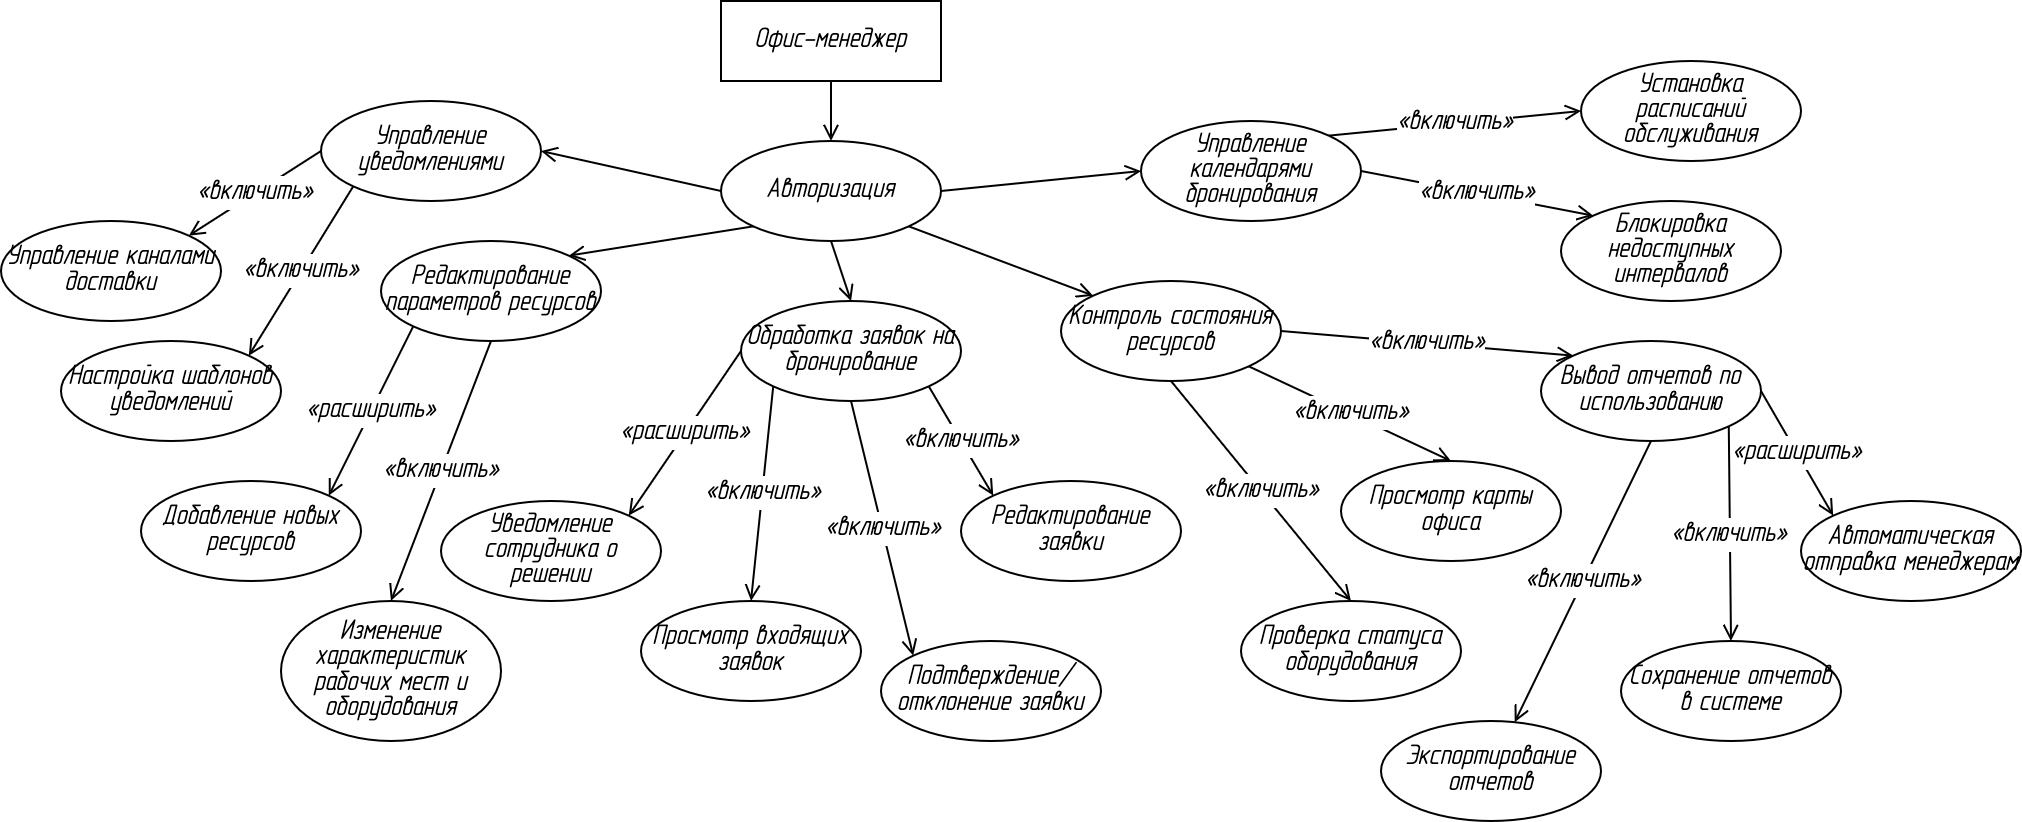
\includegraphics[width=0.99\linewidth]{assets/use-cases-office_manager.png}
            \caption{Диаграмма вариантов использования от имени офис-менеджера}
            \label{fig:tech-requirements:functional-model:use-cases-office_manager}
        \end{figure}
    \end{landscape}
    \clearpage
}


Таким образом, разработка системы управления офисными информационными процессами требует комплексного подхода к проектированию, охватывающего как функциональные, так и нефункциональные требования. Проектируемая система не только оптимизирует рабочие процессы, но и закладывает основу для дальнейшего развития корпоративной цифровой инфраструктуры, способствуя повышению продуктивности сотрудников и прозрачности управления ресурсами. Гибкость архитектуры, поддержка масштабирования и интеграция с современными средствами идентификации обеспечат стабильную и безопасную работу системы. Разработанные диаграммы показывают, что система чётко разделяет роли пользователей и предоставляет каждому только необходимый функционал. Она ориентирована на самообслуживание сотрудников и автоматизацию рутинных операций, снижая нагрузку на администраторов. Все действия проходят через механизмы согласования и контроля, что повышает управляемость офисной инфраструктурой. Наличие отчётности и повторно используемых сценариев подтверждает модульность и аналитическую направленность системы. В целом, система проектируется как масштабируемая, гибридная и удобная для работы в распределённой среде.
